\chapter{Budowa urządzenia}

\section{Konstrukcja}

Część mechaniczna urządzenia została zamodelowana w programie Solidworks, dzięki czemu ustalono jakie elementy konstrukcyjne są potrzebne oraz czy nie występują kolizje z poruszającym się wózkiem. Koncepcyjny model 3D zaprezentowano na rysunku \ref{fig:konstrukcja}. 

\begin{figure}
    \centering
    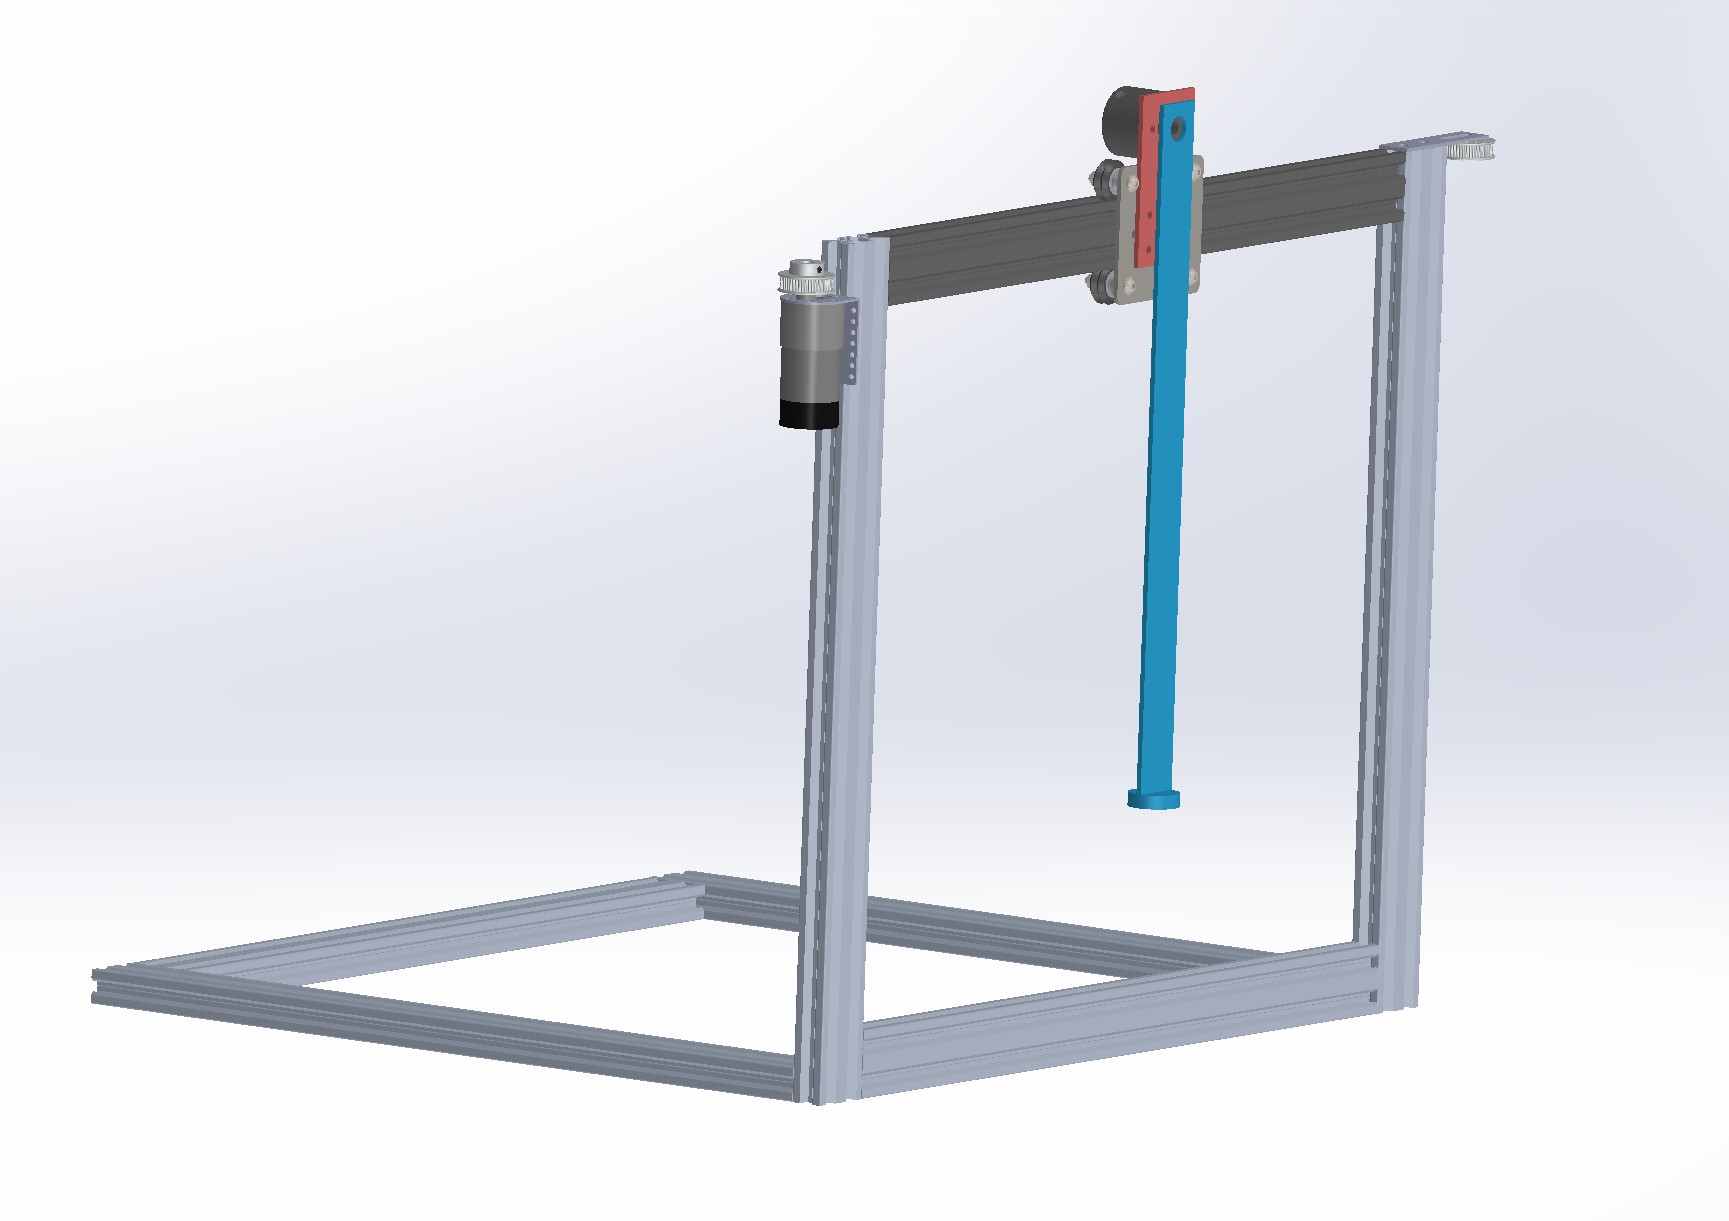
\includegraphics[scale=0.5]{praca_dyplomowa/figures/pendulum6.jpg}
    \caption{Poglądowy model 3D konstrukcji}
    \label{fig:konstrukcja}
\end{figure}

\subsection{Rama}
Do budowy konstrukcji urządzenia zostały wykorzystane aluminiowe profile typu V-Slot 2040, jak na rysunku \ref{fig:profil}. Przekrój profilu ma wymiary 20 x 40 mm, a jego boki mają charakterystyczne rowki w kształcie litery V. Rama została zbudowana z 3 profili o długości 500mm oraz 4 profili długości 250mm. Wszystkie elementy zostały ze sobą połączone dedykowanymi elementami wydrukowanymi na drukarce 3D oraz śrubami M4. Część elementów łączeniowych została znaleziona na stronie \textit{thingiverse.com}, na której udostępniane są modele 3D przygotowane z myślą o ich wydrukowaniu. Konstrukcja złożona w ten sposób charakteryzuje się dużą sztywnością, a przy tym niską masą.

\begin{figure}
    \centering
    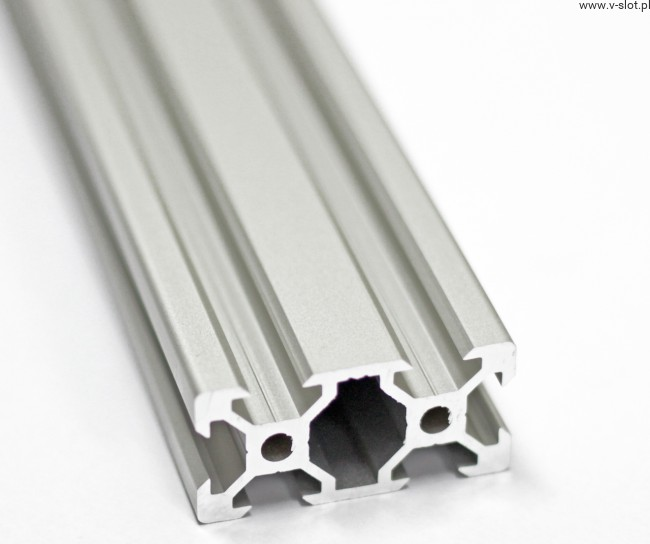
\includegraphics[scale=0.7]{praca_dyplomowa/figures/profil.jpg}
    \caption{Aluminiowy profil 2040}
    \texttt{Źródło: v-slot.pl}
    \label{fig:profil}
\end{figure}

\subsection{Układ jezdny}
Poruszający się wózek, popularnie nazywany karetką, został zbudowany na stalowej blasze, do którego przymocowano 4 łożyskowane rolki widoczne na rysunku \ref{fig:Rolka}, które są dedykowane do poruszania się po profilach V-Slot. Dodatkowo dolne rolki zostały zamontowane na tulejach mimośrodowych, dzięki czemu można regulować siłę docisku rolek do profilu. Do karetki przymocowany pas zębaty GT2 o szerokości 6mm, który z jednej strony porusza się po kole pasowym będącym napinaczem, a z drugiej po kole zębatym, które jest zamontowane na wale silnika. 

\begin{figure}
    \centering
    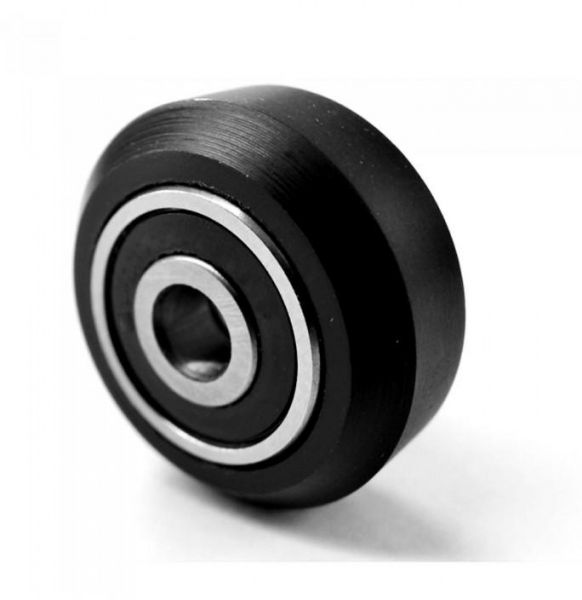
\includegraphics[scale=0.3]{praca_dyplomowa/figures/wheel.jpg}
    \caption{Rolka jezdna}
    \texttt{Źródło: black-frog.pl}
    \label{fig:Rolka}
\end{figure}
